\documentclass[11pt, oneside]{article} 
\usepackage{geometry}
\geometry{letterpaper} 
\usepackage{graphicx}
	
\usepackage{amssymb}
\usepackage{amsmath}
\usepackage{parskip}
\usepackage{color}
\usepackage{hyperref}

\graphicspath{{/Users/telliott_admin/Dropbox/Tex/png/}}
% \begin{center} 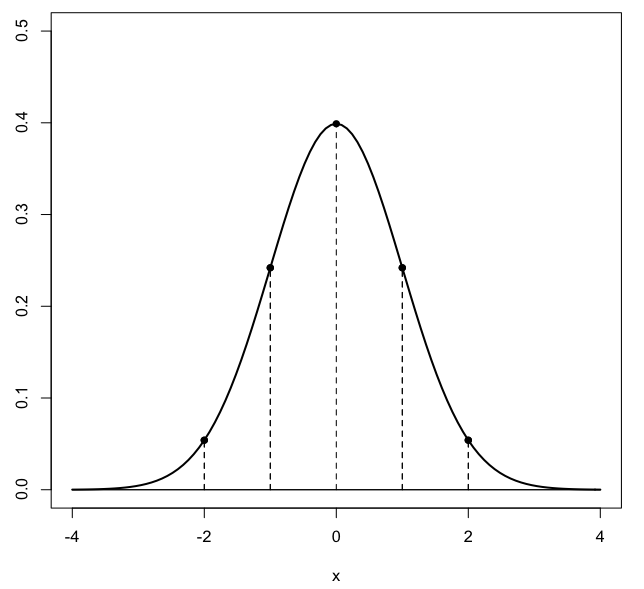
\includegraphics [scale=0.4] {gauss3.png} \end{center}

\title{Stovepipe}
\date{}

\begin{document}
\maketitle
\Large

I came across an interesting problem in a chapter of Strogatz's \emph{The Joy Of x}.  He calls it the stovepipe problem.  We want to find the volume of the region formed from the intersection of two cylinders (of equal radius), that meet at right angles.

\begin{center} 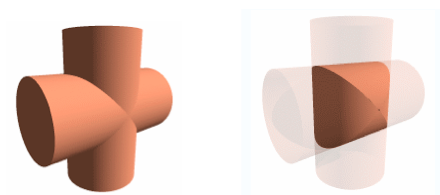
\includegraphics [scale=0.5] {stovepipe1.png} \end{center}

I really couldn't visualize it, but he told me that the horizontal cross sections of this solid are squares, and gave a picture.

\begin{center} 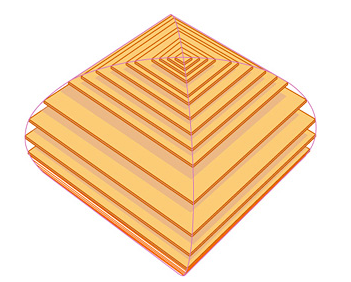
\includegraphics [scale=0.5] {stovepipe2.png} \end{center}

and it makes sense, if you imagine cutting through a potato with a cylindrical bore, then repeating at right angles.  At each level, the side is formed by cutting along the edge of the cylinder, hence the opposite sides are parallel.  And since the two cuts use the same cylinder, all $4$ sides at any particular height are equal, giving a square.

So our problem is to find the length of the side at each value of the height.  We deal with the upper half of the solid, for simplicity.  If you draw a sketch of the vertical cross-section, at each distance $h$ from the base of the solid, extending up, the remainder of the height down to the base is $R-h$, and the half-length of the side is $s/2 = \sqrt{R^2 - h^2}$.

The volume is obtained by adding up all these slices

\[ V = \int_0^R 2  \sqrt{R^2 -h^2} \ dh \]

Let's simplify the problem further (for the moment) by dealing with the case where $R=1$  We need the integral

\[ \int \sqrt{1-h^2} \ dh \]

I certainly didn't know that off the top of my head.

\[ \int \sqrt{a^2-x^2} \ dx = \frac{a^2}{2} \ [ \ \sin^{-1} \frac{x}{a} + \frac{x}{a} \sqrt{1-(\frac{x}{a})^2} \ ] \]

which can be rearranged slightly

\[ = \frac{a^2}{2} \ \sin^{-1} \frac{x}{a} + \frac{x}{2} \sqrt{a^2-x^2}  \]
for the derivation see \hyperlink{an_important_integral}{\textbf{here}}.

I'll leave it to you to figure out the whole volume for the general case with radius $R$.

\end{document}